\chapter{Encoding the Hindley-Milner type-assignment algorithm}
\label{chap:HindleyMilner}

Because Jape is based on unification, it's possible to construct a very nice version of the Hindley-Milner type-assignment algorithm, and control it in slow motion. I implemented a version of the algorithm for the lambda calculus with tuples and \textit{let} /\ textit{letrec} bindings.

\begin{ruletab}{|l|l|} 
\hline
% ROW 1
$\infer[\reason{$\lambda -I$}]
       {C |- \lambda x.E:T->T' }
       {C,x:T |- E:T' }$
& 
$\infer[\reason{$application-I$}]
       {C |- F\,G:T' }
       {C |- F:T->T' \quad C |- G:T}$ 
\\
\hline
% ROW 2
$\infer[\reason{$tuple-I$}]
       {C |- (E1,E2):(T1\times T2)}
       {C |- E1:T1\quad C |- E2:T2}$
&
$\infer[\reason{$\operatorname{let}-I$}]
       {C |- \operatorname{let}\,x=E\,\operatorname{in}\,F\,\operatorname{end}:T}
       {C |- E:T1\quad C |- T1\prec S\quad C,x:S |- F:T}$
\\
\hline
% ROW 3
\multicolumn{2}{|l|}{
$\infer[\reason{$\operatorname{letrec}-I$}]
       {C |- \operatorname{letrec}\,x=E\,\operatorname{in}\,F\,\operatorname{end}:T}
       {C,x:T1 |- E:T1\quad C |- T1\prec S\quad C,x:S |- F:T}$} 
\\
\hline
% ROW 4
$\infer[\reason{$identifier\;type$}]
       {C |- x:T}
       {C(x)\mapsto S\quad S\succ T}$
&
\\
\hline 
\end{ruletab}

In each of these rules the context $C$ is a sequence of bindings of program variables to type schemes which can be read, right to left, as a mapping from variables to type schemes. The judgement $C(x)\mapsto S$ interprets the context in just that way. The judgement $C |- T\prec S$ is the \emph{generalisation step}, in which `type variables' free in the type $T$ but not free in the context $C$ are used to transform type $T$ into type scheme $S$. The judgement $S\succ T$ is the corresponding \emph{specialisation step}, when the schematic variables of $S$ are replaced by type formulae.

The difficulties of encoding the Hindley-Milner algorithm are just those of representing the schematic `type variables', representing and interpreting the type context and implementing the generalisation and specialisation steps.

\section{Syntax}

I represent λ formulae using \textsc{leftfix}, and I give that formula a lower priority than the colon operator, so that I don't have to use too many brackets. The type-tupling operator × is treated as an associative operator, rather like comma. I need an == operator (blechh!) because = is used in the \textit{let / letrec} syntax. I use a double-arrow operator rather than a colon in the contexts, for no particularly good reason that I can remember. I have included additional operators • and ◁ which are used in the generalisation-step induction.

Type schemes which include schematic variables-- so-called polytypes --- are $@*t.T$ or $@*t1,t2.T$ and so on, with up to four schematic variables. Those which have no schematic variables --- so-called monotypes --- are \#$T$, where $T$ is a type formula. This is faithful to Milner's treatment in the ML description, where he describes the scheme $T$ as a shorthand for $@*().T$.

I have included constants \textit{hd}, \textit{tl} and \textit{nil} which are useful in describing list-processing, $\<true>$ and $\<false>$ which are useful in handling booleans; there are also constant type-names \textit{bool}, \textit{string} and \textit{num}.

Jape has no means of dividing names into distinct syntactic hierarchies: to do this algorithm properly I'd want to distinguish type variables $t$ from program variables $x$. But I can't. To keep my head straight I make two sets of declarations. First the program names:
\begin{japeish}
CLASS VARIABLE x y z e f g map\\
CLASS FORMULA E F G\\
CLASS CONSTANT c\\
CONSTANT hd tl nil\\
CLASS NUMBER n\\
CLASS STRING s\\
CONSTANT true false
\end{japeish}
and then the type names:
\begin{japeish}
CLASS VARIABLE t\\
CLASS FORMULA S T /* we use T for types, S for type schemes in the rules which follow */\\
CONSTANT bool string num
\end{japeish}
Next, operators for programs:
\begin{japeish}
SUBSTFIX\tab 500\tab \{ E / x \}\\
JUXTFIX\tab 400\\
INFIXC\tab 140L\tab + -\\
INFIXC\tab 120R\tab ::\\
INFIXC\tab 100L\tab == /* we need this because we also have let f =... */\\
LEFTFIX\tab 75\tab λ .\\
INFIX\tab 50L\tab =
\end{japeish}
\begin{japeish}
OUTFIX [ ]\\
OUTFIX letrec in end\\
OUTFIX let in end\\
OUTFIX if then else fi
\end{japeish}
and operators for types:

\begin{japeish}
INFIX\tab 150T \tab ×\\
INFIX\tab 100R \tab →\\
LEFTFIX\tab 75\tab ∀.\\
PREFIX\tab 75\tab \#\\
INFIX\tab 55L \tab • ◁\\
INFIX\tab 50L \tab : ⇒ ≺ ≻
\end{japeish}
Now bindings:

\begin{japeish}
BIND x SCOPE E IN λ x. E

BIND t SCOPE T IN ∀ t. T\\
BIND t1 t2 SCOPE T IN ∀ t1, t2. T\\
BIND t1 t2 t3 SCOPE T IN ∀ t1, t2, t3. T\\
BIND t1 t2 t3 t4 SCOPE T IN ∀ t1, t2, t3, t4. T
\end{japeish}
\begin{japeish}
BIND x \tab SCOPE F\tab IN let x = E in F end\\
BIND x1 x2 \tab SCOPE F\tab IN let x1=E1, x2=E2 in F end\\
BIND x1 x2 x3\tab SCOPE F\tab IN let x1=E1, x2=E2, x3=E3 in F end\\
BIND x1 x2 x3 x4\tab SCOPE F\tab IN let x1=E1, x2=E2, x3=E3, x4=E4 in F end\\
BIND x\tab SCOPE E F\tab IN letrec x = E in F end\\
BIND x1 x2\tab SCOPE E1 E2 F\tab IN letrec x1=E1, x2=E2 in F end\\
BIND x1 x2 x3\tab SCOPE E1 E2 E3 F\tab IN letrec x1=E1, x2=E2, x3=E3 in F end\\
BIND x1 x2 x3 x4\tab SCOPE E1 E2 E3 E4 F\tab IN letrec x1=E1, x2=E2, x3=E3, x4=E4 in F end
\end{japeish}
Finally, the definition of a judgement:
\begin{japeish}
CLASS LIST C\\
SEQUENT IS LIST ⊦ FORMULA
\end{japeish}
--- notice \textsc{list} and not \textsc{bag} as in previous chapters.

\section{Rules}

The structural rules are very straightforwardly encoded, following the algorithm directly. Note the use of a type scheme \#\textit{T1} in the rule which deals with λ formulae.
\begin{japeish}
RULE "F G : T"\tab FROM C ⊦ F: T1→T2 AND C ⊦ G : T1 \tab INFER C ⊦ F G : T2\\
RULE "λx.E : T1→T2"\tab FROM C,x⇒\#T1 ⊦ E:T2 \tab INFER C ⊦ λx.E : T1→T2\\
RULE "(E,F) : T1×T2"\tab FROM C ⊦ E: T1 AND C ⊦ F: T2\tab INFER C ⊦ (E,F) : T1×T2\\
RULE "if E then ET else EF fi : T"\\
\tab FROM C ⊦ E : bool AND C ⊦ ET : T AND C ⊦ EF : T\tab INFER C ⊦ if E then ET else EF fi : T
\end{japeish}

There are some simple rules which deal with constants:
\begin{japeish}
RULE "n:num"\tab INFER C ⊦ n:num\\
RULE "s:string"\tab INFER C ⊦ s:string\\
RULE "true:bool"\tab INFER C ⊦ true:bool\\
RULE "false:bool"\tab INFER C ⊦ false:bool
\end{japeish}
which I apply whenever possible --- in this case autounify seems to be the best mechanism:\footnote{It would be dangerous if a conclusion \_E:\_T was ever generated, but it never is.}
\begin{japeish}
AUTOUNIFY "n:num" "s:string" "true:bool" "false:bool"
\end{japeish}

Dealing with the various forms of \textit{let} and \textit{letrec} formulae is a matter of tedious listing. Here are the \textit{letrec} rules, for example:
\begin{japeish}
RULES letrecrules ARE\\
\tab FROM C,x⇒\#T1 ⊦ E:T1 AND C ⊦ T1≺S1 AND C,x⇒S1 ⊦ F:T\\
\tab \tab INFER C ⊦ letrec x=E in F end : T\\
AND\tab FROM C,x1⇒\#T1,x2⇒\#T2 ⊦ E1 : T1 AND C,x1⇒\#T1,x2⇒\#T2 ⊦ E2 : T2 \\
\tab AND C ⊦ T1≺S1 AND C ⊦ T2≺S2 AND C,x1⇒S1,x2⇒S2 ⊦ F:T\tab \\
\tab \tab INFER C ⊦ letrec x1=E1, x2=E2 in F end : T\\
AND\tab FROM C,x1⇒\#T1,x2⇒\#T2,x3⇒\#T3 ⊦ E1 : T1 AND C,x1⇒\#T1,x2⇒\#T2,x3⇒\#T3 ⊦ E2 : T2\\
\tab AND C,x1⇒\#T1,x2⇒\#T2,x3⇒\#T3 ⊦ E3 : T3 AND C ⊦ T1≺S1 AND C ⊦ T2≺S2\\
\tab AND C ⊦ T3≺S3 AND C,x1⇒S1,x2⇒S2,x3⇒S3 ⊦ F:T\\
\tab \tab INFER C ⊦ letrec x1=E1, x2=E2, x3=E3 in F end : T\\
AND\tab FROM C,x1⇒\#T1,x2⇒\#T2,x3⇒\#T3,x4⇒\#T4 ⊦ E1 : T1 \\
\tab AND C,x1⇒\#T1,x2⇒\#T2,x3⇒\#T3,x4⇒\#T4 ⊦ E2 : T2\\
\tab AND C,x1⇒\#T1,x2⇒\#T2,x3⇒\#T3,x4⇒\#T4 ⊦ E3 : T3 \\
\tab AND C,x1⇒\#T1,x2⇒\#T2,x3⇒\#T3,x4⇒\#T4 ⊦ E4 : T4\\
\tab AND C ⊦ T1≺S1 AND C ⊦ T2≺S2 AND C ⊦ T3≺S3 AND C ⊦ T4≺S4\\
\tab AND C,x1⇒S1,x2⇒S2,x3⇒S3,x4⇒S4 ⊦ F:T\\
\tab \tab INFER C ⊦ letrec x1=E1, x2=E2, x3=E3, x4=E4 in F end : T\\
END
\end{japeish}

\section{Reading the context and specialising a type scheme}

Things get more interesting when you consider how to handle the context-evaluation step $C(x)\mapsto S$ : $C$ maps variable name $x$ to scheme $S$. The context is just a list of name↦scheme bindings, and it should be read right-to-left, so that the most recent bindings take precedence. Because program names can't appear in types in this logic, I can use a notin proviso to help to read the context in this way. Because variables and constants are different syntactic classes, I need two rules:
\begin{japeish}
RULE "C ⊦ x⇒S" WHERE x NOTIN C' IS INFER C,x⇒S,C' ⊦ x⇒S\\
RULE "C ⊦ c⇒S" WHERE c NOTIN C' IS INFER C,c⇒S,C' ⊦ c⇒S
\end{japeish}
I declare these as identity rules so that their application is hidden in a box-and-line display of a proof:
\begin{japeish}
IDENTITY "C ⊦ x⇒S"\\
IDENTITY "C ⊦ c⇒S"
\end{japeish}

There is a rule for each of the constant function identifiers, binding it to a polytype or a monotype as appropriate:
\begin{japeish}
RULES constants ARE\\
\tab C ⊦ hd⇒∀tt.[tt]→tt\\
AND\tab C ⊦ tl⇒∀tt.[tt]→[tt]\\
AND\tab C ⊦ (::)⇒∀tt.tt→[tt]→[tt]\\
AND\tab C ⊦ nil⇒∀tt.[tt]\\
AND\tab C ⊦ (+)⇒\#num→num→num\\
AND\tab C ⊦ (-)⇒\#num→num→num\\
AND\tab C ⊦ (==)⇒∀tt.tt→tt→bool\\
END
\end{japeish}

Typing a variable or a constant is a matter of finding the type scheme and then specialising to some type. Specialisation is just a matter of substituting types for schematic variables:
\begin{japeish}
RULES "S≻T" ARE\\
\tab INFER \#T ≻ T\\
AND\tab INFER ∀tt.TT ≻ TT\{T1/tt\}\\
AND\tab INFER ∀tt1,tt2.TT ≻ TT\{T1,T2/tt1,tt2\}\\
AND\tab INFER ∀tt1,tt2,tt3.TT ≻ TT\{T1,T2,T3/tt1,tt2,tt3\}\\
AND\tab INFER ∀tt1,tt2,tt3,tt4.TT ≻ TT\{T1,T2,T3,T4/tt1,tt2,tt3,tt4\}\\
END
\end{japeish}
Then two rules put these together in just the way that the algorithm does:
\begin{japeish}
RULE "C ⊦ x:T" IS FROM C⊦x⇒S AND S≻T INFER C⊦x:T\\
RULE "C ⊦ c:T" IS FROM C⊦c⇒S AND S≻T INFER C⊦c:T
\end{japeish}

In the menu I use a tactic which looks in three places for a type scheme and then specialises, showing none of its working when it succeeds, but trying to give some error messages when it fails:
\begin{japeish}
TACTIC "x:T" IS
\tab SEQ \\
\tab\tab(ALT (LAYOUT "C(x)⇒S; S≻T" () "C ⊢ x:T" "C ⊢ x⇒S")  \\
\tab\tab\tab(LAYOUT "C(c)⇒S; S≻T" ()  "C ⊢ c:T" "C ⊢ c⇒S") \\
\tab\tab\tab(LAYOUT "constant" () "C ⊢ c:T" constants) \\
\tab\tab\tab(WHEN \\
\tab\tab\tab\tab(LETGOAL (\_E:\_T) \\
\tab\tab\tab\tab\tab    (Fail (x:T can only be applied to either variables or constants: you chose \_E))) \\
\tab\tab\tab\tab(LETGOAL \_E (Fail (conclusion \_E is not a ' formula:type ' judgement)))))  \\
\tab\tab"S≻T"
\end{japeish}

\section{The generalisation step}

I perform a structural induction on the type $T$ in order to calculate its schematic variables. These will be unknowns, because of course I don't judiciously introduce type variables when running the algorithm (though you can if you want to): I simply introduce unknowns as necessary.

The generalisation step is run by a tactic, and all the working is normally hidden from the user. It works with a formula \textit{type} • $\textit{scheme}_{\textit{in}}$ ◁ $\textit{scheme}_{\textit{out}}$, in which the operators • and ◁ are no more than punctuation. The starting rule is
\begin{japeish}
RULE "T≺S" IS\tab FROM C ⊦ T • \#T ◁ S \tab INFER C ⊦ T ≺ S
\end{japeish}
The induction works with rules which take a type apart, and two rules which are the base case. The structural rules are
\begin{japeish}
RULE "T1→T2•..."\tab FROM C ⊦ T1• Sin ◁ Smid AND C ⊦ T2 • Smid ◁ Sout\\
\tab \tab INFER C ⊦ T1→T2 • Sin ◁ Sout\\
RULE "T1×T2•..."\tab FROM C ⊦ T1• Sin ◁ Smid AND C ⊦ T2 • Smid ◁ Sout\\
\tab \tab INFER C ⊦ T1×T2 • Sin ◁ Sout\\
RULE "[T]•..."\tab FROM C ⊦ T • Sin ◁ Sout\\
\tab \tab INFER C ⊦ [T] • Sin ◁ Sout
\end{japeish}
The tactic applies these rules, we shall see, `by matching': they aren't allowed to make any substantial unifications which alter the problem sequent to which they are applied. So if the problem sequent is \textit{unknown} • \textit{scheme}$_{\textit{in}}$ ◁ \textit{scheme}$_{\textit{out}}$, none of the rules will be used.

The rules which deal with an unknown do so by unifying it with a freshly-minted variable name and making sure that it doesn't appear in the context or the original type:
\begin{japeish}
RULES "new t•..." (OBJECT t1) WHERE t1 NOTIN C ARE\\
\tab C⊦ t1 • \#T◁ ∀t1.T \\
AND\tab C⊦ t1 • ∀tt1.T ◁ ∀tt1,t1.T \\
AND\tab C⊦ t1 • ∀tt1,tt2.T ◁ ∀tt1,tt2,t1.T \\
AND\tab C⊦ t1 • ∀tt1,tt2,tt3.T ◁ ∀tt1,tt2,tt3,t1.T \\
END
\end{japeish}
The only formula which can possibly unify with a freshly-minted type variable is a type unknown, and these rules have a proviso that the result shouldn't be free in the context $C$. The effect is to replace an unknown type by a type variable, and by unification to include it in the context.

If none of these rules applies, then we must have an unknown which \textit{does} appear in the context: that unknown must be left alone:
\begin{japeish}
RULE "same T•..."\tab INFER C ⊦ T • S ◁ S
\end{japeish}

The whole is stitched together with a tactic which tries first the structural rules by matching, then the variable rule and finally the leave-alone rule; that tactic is used by another which starts the process, calls the induction and hides all its working:
\begin{japeish}
TACTIC geninduct IS \\
\tab ALT\tab (SEQ (MATCH (ALT "T1→T2•..." "T1×T2•...")) geninduct geninduct) \\
\tab \tab (SEQ (MATCH "[T]•...") geninduct)\\
\tab \tab "new t•..."\\
\tab \tab "same T•..."
\end{japeish}
\begin{japeish}
TACTIC generalise IS LAYOUT "generalise" () "T≺S" geninduct
\end{japeish}

We also provide a `single-step' tactic which carries out the same tasks, so that users can view the process as it evolves:
\begin{japeish}
TACTIC genstep IS \\
\tab ALT\tab "T≺S" \\
\tab \tab (MATCH "T1→T2•...") \\
\tab \tab (MATCH "T1×T2•...") \\
\tab \tab (MATCH "[T]•...") \\
\tab \tab "new t•..."\\
\tab \tab "same T•..."
\end{japeish}

\section{Automatic search}

In this chapter we are dealing with an encoding of an \textit{algorithm}, not a proper logic. It's possible to get strange answers by running the steps in the wrong order. On the other hand, it's easy to write a tactic which automatically runs the algorithm. That tactic is long-winded because it has to deal, case-by-case, with the various sizes of binding structures. If only Jape could handle families of rules...

\begin{japeish}
TACTIC Auto IS\\
\tab WHEN\tab (LETGOAL (\_x:\_T) "x:T")\\
\tab \tab (LETGOAL (\_c:\_T) \\
\tab \tab \tab (ALT\tab "x:T" "n:num" "s:string" "true:bool" "false:bool"\\
\tab \tab \tab \tab (JAPE (fail (\_c isn't a constant from the context, \\
\tab \tab \tab \tab \tab \tab \tab or one of the fixed constants))) \\
\tab \tab \tab )\\
\tab \tab )\\
\tab \tab (LETGOAL (\_F \_G:\_T) "F G : T" Auto Auto)\\
\tab \tab (LETGOAL ((\_E,\_F):\_T) "(E,F) : T1×T2" Auto Auto)\\
\tab \tab (LETGOAL ((λ\_x.\_E):\_T) "λx.E : T1→T2" Auto)\\
\tab \tab (LETGOAL (if \_E then \_ET else \_EF fi:\_T) "if E then ET else EF fi : T" Auto Auto Auto)\\
\tab \tab (LETGOAL (let \_x=\_E in \_F end:\_T) \\
\tab \tab \tab \tab letrules Auto generalise Auto)\\
\tab \tab (LETGOAL (let \_x1=\_E1, \_x2=\_E2 in \_F end:\_T) \\
\tab \tab \tab \tab letrules Auto Auto generalise generalise Auto)\\
\tab \tab ... \textit{etc...}\\
\tab \tab (LETGOAL (letrec \_x=\_E in \_F end:\_T) \\
\tab \tab \tab \tab letrecrules Auto generalise Auto)\\
\tab \tab (LETGOAL (letrec \_x1=\_E1, \_x2=\_E2 in \_F end:\_T) \\
\tab \tab \tab \tab letrecrules Auto Auto generalise generalise Auto)\\
\tab \tab ... \textit{etc...}\\
\tab \tab (LETGOAL (\_E:\_T) (JAPE (fail (\_E is not a recognisable program formula (Auto)))))\\
\tab \tab (LETGOAL \_E (JAPE (fail (\_E is not a recognisable judgement (Auto)))))
\end{japeish}

There's a similar AutoStep tactic which lets the user make just one step of the algorithm.

\begin{figure}
\centering
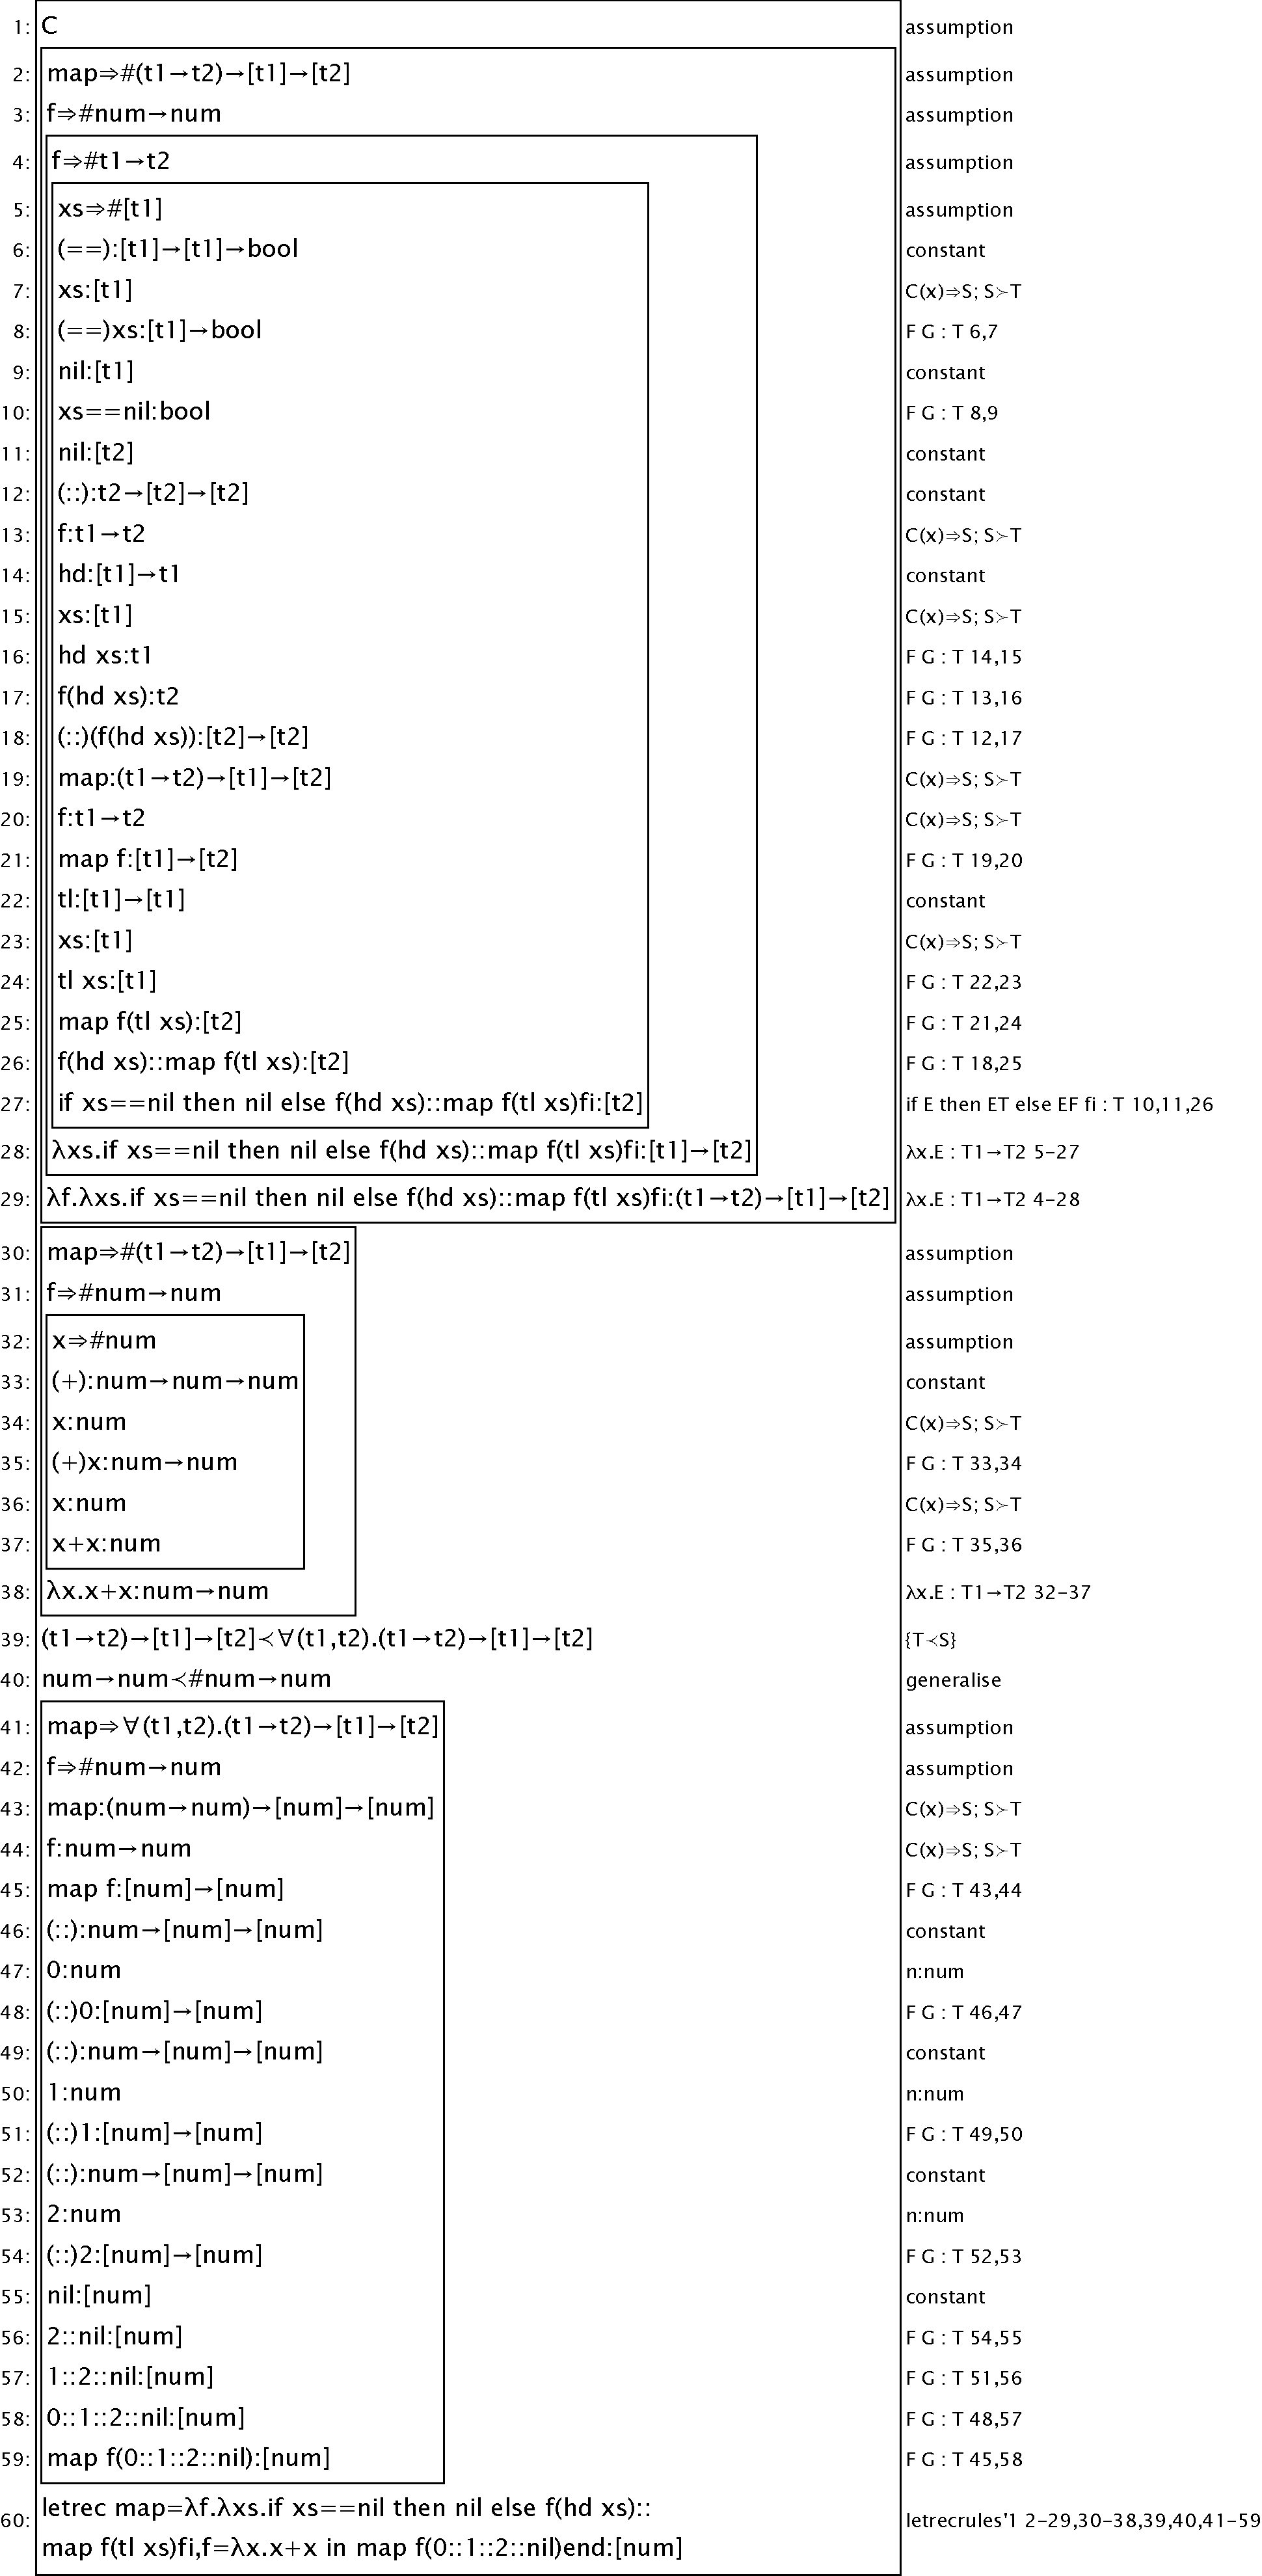
\includegraphics[scale=0.33]{pics/HindleyMilner/maptype}
\caption{A large example}
\label{fig:HindleyMilner:maptype}
\end{figure}

\section{An example}

The algorithm will calculate, for example, the type of \textit{map} and use it correctly in an application: see \figref{HindleyMilner:maptype}.

\section{Could Jape treat other type-theoretic logics?}

This encoding is a hack. It works for the simple case that it is applied to, but it shows some limitations of Jape. Conditions like `$C$ is a context' have been left out entirely, and encoding them in an interpretive tool would be pretty inefficient. Including them in rules would be tedious too. I'm aware (because Randy Pollack has several times beaten it into my head) that the `shadowing' mechanism which allows a context to be treated as a mapping isn't generally applicable.

On a more mundane level, it points up the weaknesses of the parser-generator. I can't make a distinction between program and type names (and make it stick); I have to use an ugly operator to mark monotypes in the type environment. And the fact that it doesn't deal with `families' of rules, so that you have to list all the different forms of $@*$ formulae, for example, and have a rule for each form, is very tedious.

On the other hand, though the genstep mechanism is a bit messy, it does show how it's possible to run the algorithm without resorting to guessing when to use type variables and when to use unknowns. Jape really does go through the type formula, replace replaceable unknowns with type variables, generalise the result, and get the right answer.

%In simple, `pure' logics, I can reasonably claim that Jape can transparently encode the inference rules, and all the magic is hidden in its treatment of substitutions, bindings and unification. In the case of the Hindley-Milner logic and, I expect, other type-theoretic logics, that isn't so. I've made some creative choices and had to program an encoding of the treatment of contexts. If the treatment in this chapter is to serve as a model of how Jape can encode type-theoretic logics, there are a number of questions which have to be answered.

%First, and trivially, it ought to able to deal with the monotype / polytype distinction without the ugly syntactic mechanism we have used here. That might require a more powerful parser generator.

%
%More seriously, my treatment has no judgement equivalent to `C is a context', and I have pushed the question into the context-interpretation rule, treating the context as a mapping and making sure with a proviso that Jape isn't overlooking a later binding. Meta-theoretically it is clear that the context might easily be formed by ensuring that every name it contains is distinct; the necessary alpha-conversion, however, makes it hard for a human prover to keep track of what is going on. It seems to me, therefore, that I am pragmatically correct, \emph{in this encoding}, to treat the context as a mapping. Also, the rules are context-validity preserving. But it is still possible to state a conjecture with a nonsense context and yet prove it: $\mathit{GARBAGE} |- \lambda x.x:T->T$ will be a theorem. It would be absurdly inefficient to check the validity of the context at every rule application; nevertheless, there ought to be ways in which we can check its validity at crucial points in a proof.

%
%We intend, in future work on type-theoretic logics, to continue to develop the approach used here. We expect to invent proviso mechanisms which allow us to state that the names in some type judgement are not rebound by the context to their right, or something similar. We dream, even, of user-defined provisos which will allow close control of the meaning of such provisos. We hope to find the right place to put `C is a context' judgements.
 